\documentclass[conference]{IEEEtran}
\IEEEoverridecommandlockouts
% The preceding line is only needed to identify funding in the first footnote. If that is unneeded, please comment it out.
\usepackage{cite}
\usepackage{amsmath,amssymb,amsfonts}
\usepackage{algorithmic}
\usepackage{graphicx}
\usepackage{textcomp}
\usepackage{xcolor}
\def\BibTeX{{\rm B\kern-.05em{\sc i\kern-.025em b}\kern-.08em
    T\kern-.1667em\lower.7ex\hbox{E}\kern-.125emX}}
\begin{document}

\title{Distributed Multiplayer Video Game}

\author{\IEEEauthorblockN{Ryan Wickman}
\IEEEauthorblockA{\textit{University of Memphis} \\
Memphis, USA \\
rwickman@memphis.edu}
}

\maketitle

\begin{abstract}

\end{abstract}

\section{Introduction}
In this section I will provide a brief overview of the project and its implementation details.

\subsection{Goal}
The goal of this project initially was to create a full peer-to-peer multiplayer video game.
However, due to time constraints, I switched the scope of it to mainly focus on the matchmaking Server.
Thus my goal was updated to establish a good baseline matchmaking Server that players of a Video Game could use to find and join a game session.
Although this was my goal, I still did work on other components as time allowed, details of which I will give in the next section and throughout this paper.

\subsection{Overview}
In this project, I worked on a few components of what make up a mutliplayer video game.
What this entailed was making a way for users to send information amongst one another once in the game, a matchmaking server users could use to connect to a game, and the game itself.
I decided to use a peer-to-peer architecture for the in game communication for users. 
While this may cause more latency than a dedicated, centralized server, it scales better and is more cost efficent for myself.
In this, one player is chosen to host the game and act like the server.
The rest of the players will communicate through the host user as if it was a dedicated server itself.
They will use UDP to communicate as the game is a real-time application and is thus time sensitive.
On the other hand, the matchmaking server will be centralized as there needs to be a single point for all users to connect and express interest in finding a game session to join.
The users will use TCP, as opposed to UDP, to connect to the matchmaking server as reliable data transfer is important for finding and joining a game.
The game was developed using the Unity game engine. 
It is has a main menu that users can use to find a game through the matchamking server or connect to a game directly by using an IP address of the host.
The actual gameplay is a first-person sword fighting game.
While I have a good working example for these components, this is far from the final product it will eventually be.
Thus throughout this paper I will provide incite to where I beleive the application could be improved or expanded on.

\section{Matchmaking Server}
The majority of the time I spend on this project was focused on the matchmaking server.
It ended up having a lot more moving components than I first anticipated.
I used C++ to code everything and CMake to manage the build procces, and I used Boost.Asio to provide asynchronous networking capability.
The server is made up of a few parts: matchmaking server interface, TCPConnection, and game queue.

\subsection{Packet}
In the exchanging of information between independent applications there needs to be a uniform way for the to pass and read message in support of interoperability. 
Such a requirement requires an agreement between the communicating applications such as them both following a specific protocol.
Due to this, I created my own packet types that the front-end video game programmed in C# can use to communicate with the backend matchmaking server programmed in C++.  
The packets carry data that is created by one side and  consumed by the other side.
The data in the packets are in JSON data format, which uses key-value pairs.  
This has to be serialized before it is sent over the network and deserialized when it arrives to its destination.
The reason I chose this data format is because there are libraries in both C# and C++ that support the use of this data format and it is rather ease of use of JSON.

The packets themselves were designed to be lightweight and easily extensible.
There are a many different packet types I created throughout this project; I will give a description of all of them later on in this section.
They all inherit from the parent class Packet and have the naming scheme of "<packet type>Packet".
The Packet class has member variables for the header length, maximum body length, body length, a char array to store the data, and a packet type.
The header length is the fixed amount of bytes contained in the header.
The maximum body length is the upper limit for the amount of bytes that can be contained in  a packet.
The body length is the amount of bytes contained in the body.
The data char array is where the header and body are actually stored.
This is also what is actually send over the network when communicating.
The header is the first 8 character of the data array and it contains the body length.
The reason for having a header store this information is because the body of a packet differs between packet types.
Furthermore, it allows for variable length packets which thus provides more granularity of the data sent and reduces wasted bandwidth consumption.
The body of the packet is what contains the actual payload of the packet: the serialized JSON data.
This JSON data differs between packet types; however, all of them contain the key-value pair for the packet type.

The Packet class also has member functions to access its protected members, to decode and encode the header, to decode the body, and to encode both the header at once body.
The functions to access the protected members include data(), body(), length(), body\textunderscore length(), and packet\textunderscore type().
All of these are pretty much self explanitory given their names.
The only interesting one is Packet::body() which returns data\textunderscore + header\textunderscore length.
The reason for doing this is because of pointer arithmetic in C++, this will return a pointer to the first char in the body.

The function Packet::set\textunderscore body\textunderscore length is used to set the body length of the packet, but will cap it at the maximum body length if an attempt is made to exceed this upper limit.
The function Packet::encode\textunderscore header() is used to serialize the packet header.
First, it creates a temporary char array called header of size header length + 1.
Then, It then writes the body length to this char array,
Finally, it copies the bytes in this char array to the data member variable.

The function Packet::decode\textunderscore header is what is used to decode the serialized header that is stored in the member data array.
It return a boolean indicated if the it was successful in decoding the header.
First, it creates a temporary char array called header of size header length + 1.
Then, it copies the first 8 bytes of the data array into the header array.
Next, it sets the body length to the integer represented by this array of chars.
Finally, if the body length is greater than the max body length it sets body length equal to 0 and returns false.
If the body length is less than or equal to the max body length it returns true.

As you may notice I have yet to explain the functions for decoding and encoding the body.
This is because they are pure virtual as to enforce the children classes to provide their own implementation to encode and decode the body. 
The reason for doing this is because the information contained in the body of a packet differs between packet types.
Now I shall explore the classes that inherit from Packet.

The class FindPacket is what is used when a user wants to join a game.
It contains two additional members variables for a unique identifier for the client and the game type the user wants to join.
It also has additional member function for accessing the members and the implementation details for encode and decode\textunderscore body.
The FindGamePacket::encode function is used to serialize the member variables of the class and the header so it can be sent over the network.
First, it creates a JSON data type.
I am using a library called nlohmann to achieve this.
Second, It sets the key-value pairs for the packet type, user ID, and game type.
Third, it serializes the JSON data and stores it in a string called find\textunderscore game\textunderscore str.
Fourth, it calls set\textunderscore body\textunderscore length with the size of find\textunderscore game\textunderscore str as its argument.
Fifth, it encodes the header.
Finally, it copies find\textunderscore game\textunderscore str to the body of the packet.

The  FindGamePacket::decode\textunderscore body function is what is used to decode the body for use of the receiver of the packet.
First, it deserializes the data by parsing it into a JSON object called find\textunderscore game\textunderscore json.
Second, it sets the member variables to the values of find\textunderscore game\textunderscore json.

For this instance I gave an explanation of Packet::encode and Packet::decode\textunderscore body; however. for the rest of the packet types I will not give one as the implementation is extremely similar.
The only differences include getting and setting the unique member variables for each packet types.


The JoinPacket class is provided by a host a game session to client users whom want to join the game. 
It contains information required by the users to join said game.
The two member variables it contains is the IP address of the host and the PID of the game session.

The HostPacket class is used by the GameQueue to tell a user to host a game.
The only member variable it contains is the game type the user needs to create a session of.

The AckPacket class is used to keep the TCP connection alive while the users is waiting to join or host a game.
I will give more details to this later and why it is necessary in the TCPConnection section.
It contains member variables for the ack type,
This ack type is of type AckType which is an enum defined in the ack\textunderscore type.hpp file.
It currently only has two possible values None and Error.
The ack\textunderscore type.hpp file also includes a class called ack\textunderscore error.
This is used when the value of ack type is set to Error.

Nonetheless that finishes the discussion on the different packet types and their individual usage.
I will go into more detail later on how each one is used in the matchmaking server setting.


\subsection{Mathmaking Server Interface}
This is the point in which the user will first connect to the server.
The server is listening on a specified port and accepts incoming requests when the arrive. 
It asynchronously accepts the requests then initiates a callback that handles setting up the TCP socket to the client.
This allows for multiple users to connect to the server at once. 
The socket is constructed by initializing a TCPConnection object that will handle the rest of the users communication to find a game.
While I did consider creating a new thread for each connection, I did not due to time constraints and not wanting to deal with the complexity of adding multithreading such as locking resources, race conditions, ect..
When I update this application in the future I will potentially add this feature.

\subsection{TCPConnection}
The bulk of my time that I spent on the matchmaking server was on the TCPConnection class.
This is due to many factors such as redesigns, updating call sequences, callbacks, and simply just the overall complexity of this component.
The job of this component pertains  to handling the communication with the user that allows them to connect to a game.
This is done through a series of callback functions that create asynchronous read and write operations.
In the previous sections I explained each member of the class in no particular order, however in this one I will explain them as I go through the process of how it works.

The first think that occurs is the TCPConnection object is instantiated when a user connects to the server.
The TCPConnection is created by factory method aptly named create.
This function has two parameters for a boost::asio::io\textunderscore context reference called io\textunderscore context and a GameQueueManager reference called game\textunderscore queue\textunderscore manager.
`I calls the private constructor for TCPConnection and returns a shared pointer to the created object. 
The parameter  io\textunderscore context is used to create  an I/O object of type boost::asio::ip::tcp::socket called socket\textunderscore .
The member variable socket\textunderscore  is used throughout the TCPConnection object to perform the asynchronous write and read operations.
The other parameter, the GameQueueManager reference, is used to populate a member variable game\textunderscore queue\textunderscore manager\textunderscore .
This is used to get the game queue of specific type, I will go into more detail on this later.

After the TCPConnection object is created, its start function is called.
The function TCPConnection::start only does one thing: call TCPConnection::do\textunderscore read\textunderscore find\textunderscore game\textunderscore header.

The function TCPConnection::do\textunderscore read\textunderscore find\textunderscore game\textunderscore header is used to read the header of the FindGamePacket that will be sent by the user.
First, it  set the local variable self to the result of the call share\textunderscore from\textunderscore this() which returns a shared\textunderscore ptr<TCPConnection> object that shares ownership of *this.


Second, it will start the asynchronous operation by calling boost::asio::async\textunderscore read.
The arguments to this function include the TCP socket object, the buffer to read the data into, a callback function to be fired once the read operation completes.
The buffer is created from the data  char array  of a member variable of type FindGamePacket called find\textunderscore game\textunderscore packet  and its header length, 8 bytes.
The callback function is a lambda function that captures this and the self variable created earlier and takes in parameters that are populated by Boost.Asio when the read operation completes.
These parameters are boost::system::error\textunderscore code ec and std::size\textunderscore t length.
The ec variable indicated whether an error occurred and the length is how much data was read, in this case should be 8 bytes unless an error occurs.
Now after this operation is requested, the TCP connection stays alive until this operation is complete.
The reason for this being that shared pointer to *this is passed to the callback function of the asynchronous read.
The TCPConnection object cannot be destroyed until the last shared pointer reference is destroyed.
When the header of the FindGamePacket header is read, the callback is fired.
The callback first checks has not occurred and if it can successfully decode the FindGamePacket header.
If both of these are true, then TCPConnection::do\textunderscore read\textunderscore find\textunderscore game\textunderscore body is called.
If not, then the TCP socket  is closed.

The function TCPConnection::do\textunderscore read\textunderscore find\textunderscore game\textunderscore body reads the body of the FindGamePacket from the client.
It is similar to what occurs in TCPConnection::do\textunderscore read\textunderscore find\textunderscore game\textunderscore body so I will skip some of the details.
Once the body is read the callback function for this asynchronous read operation commences.
First, it decodes the body of the packet.
Second, it uses the game\textunderscore queue\textunderscore manager\textunderscore  member variable to get the game queue for the game type specified in the FindGamePacket object.
Third, if both the previous steps are successful, it will create a User object using the user ID from the FindGamePacket instance, the IP address from the socket, TCPConnection::host\textunderscore game, and TCPConnection::join\textunderscore game. 
Fourth, it will push this created the created User instance on the queue.
Fifth, it will call TCPConnection::do\textunderscore read\textunderscore ack\textunderscore header.


\subsection{Game Queue}
Before a user is able to join a game session, they need to wait their turn so that everyone who came in before them has the chance to join a game. 
This is why I went with a FIFO data structure such as a queue to implement this feature. 
However, in a video game with multiple game types, a user may only want to join a specific one.
Thus, it would not make sense for users looking for different game types to be in the same queue.
My solution to these requirements is to have a GameQueue superclass that is inherited from by all queues handling the users of a specific game type. \par
This class has members variables for the queue that stores weak pointers to Users, an unordered user map, the game type of this queue, the minimum and maximum size of a game session, the current queue size, and a boolean flag for if a game is currently getting prepared.
The queue is a std::queue that simply stores std::weak\textunderscore ptr<User> types. The reason it stores this type and not a User directly is because a connection may get dropped while a user is in queue.
If this occurs, then the queue will be able to correctly verify this by checking if the User object the pointer points to is expired before it uses it.
The user map is used to keep track of the amount of times a user has been added to a queue.
This, however, is not to prevent duplicate entries in the queue, but to make sure the user’s place in the queue is updated.
For example, once a game is initiated and a user is popped from the queue it will need to verify its count is equal to 1 to add it the game session.
If its count in this maps is greater than 1, then it will decrement this count and go on to the next user in the queue.
If its count is 0 then it assumed this user was erased from the queue and it does nothing.
You might be thinking what is the point of all this and why not just remove the user from the queue when a duplicate is detected or if an erase is called?
Initially I did think about doing this.
However, for many reasons I decided against it.
For one, on average it takes O(1) time to look up an element in a map, while it takes O(n) to erase an element from a queue.
So it is faster.
Albeit, it does add extra space complexity of O(n) so there is a bit of a trade off.
Additionally, in the future when introduce multithreading to this application, race conditions will begin to be an issue.
If I was to erase an element from the queue while concurrently trying to pop an element out undefined behavior may occur.
To prevent this, the queue would have to be locked until the erase finishes.
Instead a simple update to the user map will not effect the queue operation.
The worst case scenario is a user is added to a game before they should be because they were removed from the queue before the user map could update their count.
This of course could also be fixed by locking the queue, but would take less time on average due to the smaller time complexity.
The current queue size is used to keep track of the amount of unique users in the queue.
This will always be less than or equal to the actual queue size as there could be duplicate users in the queue.
The game type of the game queue is represented as an enum value.
I have a file, game\textunderscore type.hpp, specifying all the possible game types as an enum.

There are also several member functions in the GameQueue class: push, pop, erase, prepare\textunderscore game, and start\textunderscore game.
They are all pure virtual function as it is up to the inheriting class to define their behavior.
This of course makes the GameQueue class abstract, and thus I only have the GameQueue header and not associated cpp implementation file.
Currently, due to time constraints,  I only have one game type called deathmatch.
Its class is aptly named DeathmatchGameQueue.
All future GameQueue children will follow this naming convention of "<game type>GameQueue".
This class has same the members as the GameQueue superclass, albeit, with its own unique implementation of member functions of which I will explain in depth.

The DeathmatchGameQueue::push function has a single parameter of type std::shared\textunderscore ptr<User>& aptly named user.
This is what is being requested to be added to the queue.
First, it will see if the user has already been added to the queue by checking if the user ID is in the user map.
If it is not, it is inserted in the user map with a count of 1 and increment the queue size.
If it is in the queue, but its count is less than 0 meaning its been erased from the queue but not yet popped off, then it will set its count to 1 and increment the queue size.
If it is already in the queue and its count is greater than 1 then it will only increment its count. 
After checking its count, the user is added to the queue.
Finally, if with this added users queue size made it large enough to start a game and a game is already not getting prepared it will call DeathmatchGameQueue::prepare\textunderscore game.

The DeathmatchGameQueue::pop function is a little more complicated than I initially hoped.
This is due to the unforeseen complexity of having duplicates in the queue and the potential of having a user whose connection is closed in the queue.
When the pop function is called, it will first check if the current queue size is less than or equal to 0.
If it is, it will return a default weak\textunderscore ptr that points at nothing, so pretty much just null.
Then, if queue size is greater than 0, it will keep trying to get a user off the queue until it find a user that still has an active connection.
If no such user is found it will return weak\textunderscore ptr<User>().
Now, once a user is found, it will check if the user is duplicated in the queue.
If it is, it will pop out users out of the queue until it finds one that is not duplicated.
When duplicates are removed in this way, their count is decremented.
Finally, once a nonduplicated, alive user is found it will erase it from the user map, decrement the queue size, and return a weak pointer to the user.

The DeathmatchGameQueue::erase function is rather simple.
It first checks if the user is in the user map.
If it is, then it is removed from the user map and the queue size is decremented.
This operation is again O(1) on average rather than O(n) and thus the erase function becomes O(1) on average.

The DeathmatchGameQueue::prepare\textunderscore game function is what I said earlier is called once the queue reaches a certain minimum size.
Firstly, it will set a boolean flag to true to indicate a game is getting prepared.
Secondly, the user in the front is popped off the queue.
Thirdly, it will call the host\textunderscore callback function on the user passing in a reference to DeathmatchGameQueue::start\textunderscore queue function and the game type of this queue.

The DeathmatchGameQueue::star\textunderscore game function is used as a callback that is fired by the TCPConnection object of a host of a game once it is ready for users to join the game it is hosting.
It has a single parameter for a JoinPacket.
First, the packet is encoded, which serializes the packet to get ready to be sent over the wire to the user.
Then, the it will enter in a while loop that will continue as long as a maximum amount of users have been added or the queue is empty.
Next, inside this loop a user is popped of this queue, the current game size is incremented, and the join\textunderscore callback on the user is called with the JoinPacket object passed as an argument.
Finally, the preparing game flag is set to false.

Now that wraps up the implementation and design of the game queue.

\subsection{User}
The User class was created so that an item could be added to the game queue that is representative of a unique user.
Additionally, it contains smart pointers that contain references for callback functions that are used to allow the user to join or host a game.
Originally I planned on having a reference to the TCPConnection object in the User class.
However, the problem to this is it would create a circular dependency with the GameQueue class.
This is because the GameQueue class includes the header for the User class declarations and the TCPConnection includes the header for the GameQueue class declarations.
So, instead the User has reference to the functions "TCPConnection::host\textunderscore game and "TCPConnection::host\textunderscore game" to prevent such a circular dependency, but still have the necessary functionality.
This also provides more control for the TCPConnection to decide and handle what exact functions gets called.
In the future, this may prove helpful if I require different users to behave differently when joining or hosting a game.
One such instance would be if a private game is being created where only select users are able to join.
This join callback could provide additional authentication statements to verify a user can join a game before making a failed attempt and the TCPConnection closing thinking the user found a game.

\begin{figure}[h]
\centerline{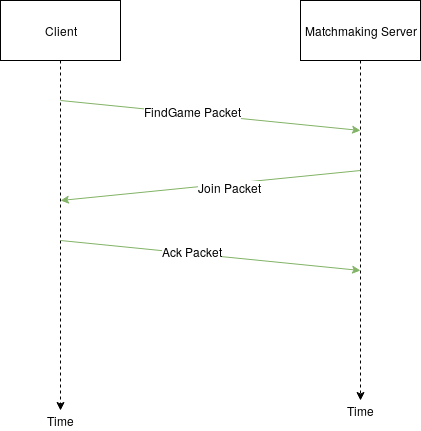
\includegraphics[width=\linewidth, height=6cm]{figures/ClientCommunication.png}}
\caption{An example of communication that will occur when a user will act as a client in the game session }
\label{fig}
\end{figure}

\begin{figure}[h]
\centerline{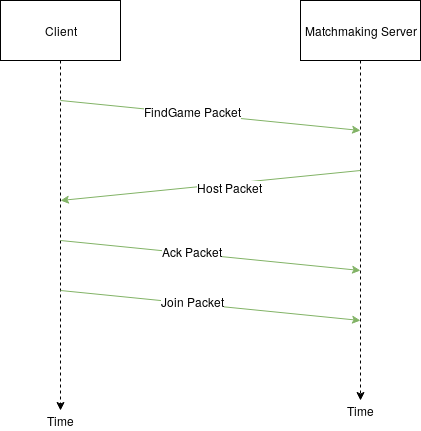
\includegraphics[width=\linewidth, height=6cm]{figures/HostCommunication.png}}
\caption{An example of communication that will occur when a user will act as a client in the game session. }
\label{fig}
\end{figure}


\section{Prepare Your Paper Before Styling}
Before you begin to format your paper, first write and save the content as a 
separate text file. Complete all content and organizational editing before 
formatting. Please note sections \ref{AA}--\ref{SCM} below for more information on 
proofreading, spelling and grammar.

Keep your text and graphic files separate until after the text has been 
formatted and styled. Do not number text heads---{\LaTeX} will do that 
for you.

\subsection{Abbreviations and Acronyms}\label{AA}
Define abbreviations and acronyms the first time they are used in the text, 
even after they have been defined in the abstract. Abbreviations such as 
IEEE, SI, MKS, CGS, ac, dc, and rms do not have to be defined. Do not use 
abbreviations in the title or heads unless they are unavoidable.

\subsection{Units}
\begin{itemize}
\item Use either SI (MKS) or CGS as primary units. (SI units are encouraged.) English units may be used as secondary units (in parentheses). An exception would be the use of English units as identifiers in trade, such as ``3.5-inch disk drive''.
\item Avoid combining SI and CGS units, such as current in amperes and magnetic field in oersteds. This often leads to confusion because equations do not balance dimensionally. If you must use mixed units, clearly state the units for each quantity that you use in an equation.
\item Do not mix complete spellings and abbreviations of units: ``Wb/m\textsuperscript{2}'' or ``webers per square meter'', not ``webers/m\textsuperscript{2}''. Spell out units when they appear in text: ``. . . a few henries'', not ``. . . a few H''.
\item Use a zero before decimal points: ``0.25'', not ``.25''. Use ``cm\textsuperscript{3}'', not ``cc''.)
\end{itemize}

\subsection{Equations}
Number equations consecutively. To make your 
equations more compact, you may use the solidus (~/~), the exp function, or 
appropriate exponents. Italicize Roman symbols for quantities and variables, 
but not Greek symbols. Use a long dash rather than a hyphen for a minus 
sign. Punctuate equations with commas or periods when they are part of a 
sentence, as in:
\begin{equation}
a+b=\gamma\label{eq}
\end{equation}

Be sure that the 
symbols in your equation have been defined before or immediately following 
the equation. Use ``\eqref{eq}'', not ``Eq.~\eqref{eq}'' or ``equation \eqref{eq}'', except at 
the beginning of a sentence: ``Equation \eqref{eq} is . . .''

\subsection{\LaTeX-Specific Advice}

Please use ``soft'' (e.g., \verb|\eqref{Eq}|) cross references instead
of ``hard'' references (e.g., \verb|(1)|). That will make it possible
to combine sections, add equations, or change the order of figures or
citations without having to go through the file line by line.

Please don't use the \verb|{eqnarray}| equation environment. Use
\verb|{align}| or \verb|{IEEEeqnarray}| instead. The \verb|{eqnarray}|
environment leaves unsightly spaces around relation symbols.

Please note that the \verb|{subequations}| environment in {\LaTeX}
will increment the main equation counter even when there are no
equation numbers displayed. If you forget that, you might write an
article in which the equation numbers skip from (17) to (20), causing
the copy editors to wonder if you've discovered a new method of
counting.

{\BibTeX} does not work by magic. It doesn't get the bibliographic
data from thin air but from .bib files. If you use {\BibTeX} to produce a
bibliography you must send the .bib files. 

{\LaTeX} can't read your mind. If you assign the same label to a
subsubsection and a table, you might find that Table I has been cross
referenced as Table IV-B3. 

{\LaTeX} does not have precognitive abilities. If you put a
\verb|\label| command before the command that updates the counter it's
supposed to be using, the label will pick up the last counter to be
cross referenced instead. In particular, a \verb|\label| command
should not go before the caption of a figure or a table.

Do not use \verb|\nonumber| inside the \verb|{array}| environment. It
will not stop equation numbers inside \verb|{array}| (there won't be
any anyway) and it might stop a wanted equation number in the
surrounding equation.

\subsection{Some Common Mistakes}\label{SCM}
\begin{itemize}
\item The word ``data'' is plural, not singular.
\item The subscript for the permeability of vacuum $\mu\textunderscore {0}$, and other common scientific constants, is zero with subscript formatting, not a lowercase letter ``o''.
\item In American English, commas, semicolons, periods, question and exclamation marks are located within quotation marks only when a complete thought or name is cited, such as a title or full quotation. When quotation marks are used, instead of a bold or italic typeface, to highlight a word or phrase, punctuation should appear outside of the quotation marks. A parenthetical phrase or statement at the end of a sentence is punctuated outside of the closing parenthesis (like this). (A parenthetical sentence is punctuated within the parentheses.)
\item A graph within a graph is an ``inset'', not an ``insert''. The word alternatively is preferred to the word ``alternately'' (unless you really mean something that alternates).
\item Do not use the word ``essentially'' to mean ``approximately'' or ``effectively''.
\item In your paper title, if the words ``that uses'' can accurately replace the word ``using'', capitalize the ``u''; if not, keep using lower-cased.
\item Be aware of the different meanings of the homophones ``affect'' and ``effect'', ``complement'' and ``compliment'', ``discreet'' and ``discrete'', ``principal'' and ``principle''.
\item Do not confuse ``imply'' and ``infer''.
\item The prefix ``non'' is not a word; it should be joined to the word it modifies, usually without a hyphen.
\item There is no period after the ``et'' in the Latin abbreviation ``et al.''.
\item The abbreviation ``i.e.'' means ``that is'', and the abbreviation ``e.g.'' means ``for example''.
\end{itemize}
An excellent style manual for science writers is \cite{b7}.

\subsection{Authors and Affiliations}
\textbf{The class file is designed for, but not limited to, six authors.} A 
minimum of one author is required for all conference articles. Author names 
should be listed starting from left to right and then moving down to the 
next line. This is the author sequence that will be used in future citations 
and by indexing services. Names should not be listed in columns nor group by 
affiliation. Please keep your affiliations as succinct as possible (for 
example, do not differentiate among departments of the same organization).

\subsection{Identify the Headings}
Headings, or heads, are organizational devices that guide the reader through 
your paper. There are two types: component heads and text heads.

Component heads identify the different components of your paper and are not 
topically subordinate to each other. Examples include Acknowledgments and 
References and, for these, the correct style to use is ``Heading 5''. Use 
``figure caption'' for your Figure captions, and ``table head'' for your 
table title. Run-in heads, such as ``Abstract'', will require you to apply a 
style (in this case, italic) in addition to the style provided by the drop 
down menu to differentiate the head from the text.

Text heads organize the topics on a relational, hierarchical basis. For 
example, the paper title is the primary text head because all subsequent 
material relates and elaborates on this one topic. If there are two or more 
sub-topics, the next level head (uppercase Roman numerals) should be used 
and, conversely, if there are not at least two sub-topics, then no subheads 
should be introduced.

\subsection{Figures and Tables}
\paragraph{Positioning Figures and Tables} Place figures and tables at the top and 
bottom of columns. Avoid placing them in the middle of columns. Large 
figures and tables may span across both columns. Figure captions should be 
below the figures; table heads should appear above the tables. Insert 
figures and tables after they are cited in the text. Use the abbreviation 
``Fig.~\ref{fig}'', even at the beginning of a sentence.

\begin{table}[htbp]
\caption{Table Type Styles}
\begin{center}
\begin{tabular}{|c|c|c|c|}
\hline
\textbf{Table}&\multicolumn{3}{|c|}{\textbf{Table Column Head}} \\
\cline{2-4} 
\textbf{Head} & \textbf{\textit{Table column subhead}}& \textbf{\textit{Subhead}}& \textbf{\textit{Subhead}} \\
\hline
copy& More table copy$^{\mathrm{a}}$& &  \\
\hline
\multicolumn{4}{l}{$^{\mathrm{a}}$Sample of a Table footnote.}
\end{tabular}
\label{tab1}
\end{center}
\end{table}

Figure Labels: Use 8 point Times New Roman for Figure labels. Use words 
rather than symbols or abbreviations when writing Figure axis labels to 
avoid confusing the reader. As an example, write the quantity 
``Magnetization'', or ``Magnetization, M'', not just ``M''. If including 
units in the label, present them within parentheses. Do not label axes only 
with units. In the example, write ``Magnetization (A/m)'' or ``Magnetization 
\{A[m(1)]\}'', not just ``A/m''. Do not label axes with a ratio of 
quantities and units. For example, write ``Temperature (K)'', not 
``Temperature/K''.

\section*{Acknowledgment}

The preferred spelling of the word ``acknowledgment'' in America is without 
an ``e'' after the ``g''. Avoid the stilted expression ``one of us (R. B. 
G.) thanks $\ldots$''. Instead, try ``R. B. G. thanks$\ldots$''. Put sponsor 
acknowledgments in the unnumbered footnote on the first page.

\section*{References}

Please number citations consecutively within brackets \cite{b1}. The 
sentence punctuation follows the bracket \cite{b2}. Refer simply to the reference 
number, as in \cite{b3}---do not use ``Ref. \cite{b3}'' or ``reference \cite{b3}'' except at 
the beginning of a sentence: ``Reference \cite{b3} was the first $\ldots$''

Number footnotes separately in superscripts. Place the actual footnote at 
the bottom of the column in which it was cited. Do not put footnotes in the 
abstract or reference list. Use letters for table footnotes.

Unless there are six authors or more give all authors' names; do not use 
``et al.''. Papers that have not been published, even if they have been 
submitted for publication, should be cited as ``unpublished'' \cite{b4}. Papers 
that have been accepted for publication should be cited as ``in press'' \cite{b5}. 
Capitalize only the first word in a paper title, except for proper nouns and 
element symbols.

For papers published in translation journals, please give the English 
citation first, followed by the original foreign-language citation \cite{b6}.

\begin{thebibliography}{00}
\bibitem{b1} G. Eason, B. Noble, and I. N. Sneddon, ``On certain integrals of Lipschitz-Hankel type involving products of Bessel functions,'' Phil. Trans. Roy. Soc. London, vol. A247, pp. 529--551, April 1955.
\bibitem{b2} J. Clerk Maxwell, A Treatise on Electricity and Magnetism, 3rd ed., vol. 2. Oxford: Clarendon, 1892, pp.68--73.
\bibitem{b3} I. S. Jacobs and C. P. Bean, ``Fine particles, thin films and exchange anisotropy,'' in Magnetism, vol. III, G. T. Rado and H. Suhl, Eds. New York: Academic, 1963, pp. 271--350.
\bibitem{b4} K. Elissa, ``Title of paper if known,'' unpublished.
\bibitem{b5} R. Nicole, ``Title of paper with only first word capitalized,'' J. Name Stand. Abbrev., in press.
\bibitem{b6} Y. Yorozu, M. Hirano, K. Oka, and Y. Tagawa, ``Electron spectroscopy studies on magneto-optical media and plastic substrate interface,'' IEEE Transl. J. Magn. Japan, vol. 2, pp. 740--741, August 1987 [Digests 9th Annual Conf. Magnetics Japan, p. 301, 1982].
\bibitem{b7} M. Young, The Technical Writer's Handbook. Mill Valley, CA: University Science, 1989.
\end{thebibliography}
\vspace{12pt}
\color{red}
IEEE conference templates contain guidance text for composing and formatting conference papers. Please ensure that all template text is removed from your conference paper prior to submission to the conference. Failure to remove the template text from your paper may result in your paper not being published.

\end{document}
